\chapter{Modelo de comportamiento de conductor}
\label{ch:behavior-model}

\section{Introducción}

\TODO{no sé qué poner}

\TODO{Hablar del esquema general (a muy grandes rasgos) del modelo de conducción que se pretende conseguir. Por qué es así, por qué queremos esas salidas y qué limitaciones nos impone el simulador sobre el que trabajamos. Aunque SUMO es continuo en el espacio, vamos sobre raíles.}

El modelo será entrenado siguiendo un esquema supervisado, por lo que necesitamos datos reales a partir de los cuales deberá ajustar su funcionamiento.

La información que se considera suficiente para que los modelos desempeñen su función en el entorno de simulación y la razón por la cual se ha tenido en cuenta es la siguiente:

\begin{itemize}
	\item \textbf{Entorno} El conductor, y por tanto el modelo, desarrolla su actividad y basa sus comportamientos, entre otros factores, en el entorno en el que se encuentra inmerso. Se considera por tanto que el ajuste de la velocidad y, sobre todo los cambios de carril, se ven influenciados por éste.
	\item \textbf{Velocidad actual del vehículo y velocidad máxima del carril}. Tanto la velocidad en la vía como del vehículo en un momento concreto influye en cómo el conductor va a modificar su aceleración en momentos posteriores.
	\item \textbf{Distancia y diferencia de velocidad con el vehículo delantero}. Al igual que con la velocidad, el vehículo delantero juega un papel esencial en los cambios de aceleración. También se intuye que puede influir en el comportamiento de cambio de carril en casos en los que el vehículo delantero va muy lento
	\item \textbf{Siguiente salida y carriles cortados}. Se considera que este tipo de información es crucial a la hora de realizar cambios de carril, ya que además de lo obvio, puede influir en otras maniobras tales como un adelantamiento.
	\item \textbf{Señales}. Es interesante contar con este tipo de señales ya que pueden influir en diferentes patrones de aceleración (e.g. estamos cerca y cambia de color a ámbar) o desaceleración (e.g. aproximación a un ceda el paso, stop o semáforo en rojo).
\end{itemize}

\section{Extracción de datos de conducción}

Se ha hecho uso de un vehículo instrumentado con sensores para capturar la mayor cantidad posible de información especificada en la introducción. El vehículo en cuestión es un Mitsubishi iMiEV (Figura~\ref{fig:instrumented-imiev}) y los dispositivos un LIDAR, un GPS, el Bus CAN y una cámara.

\begin{figure}
	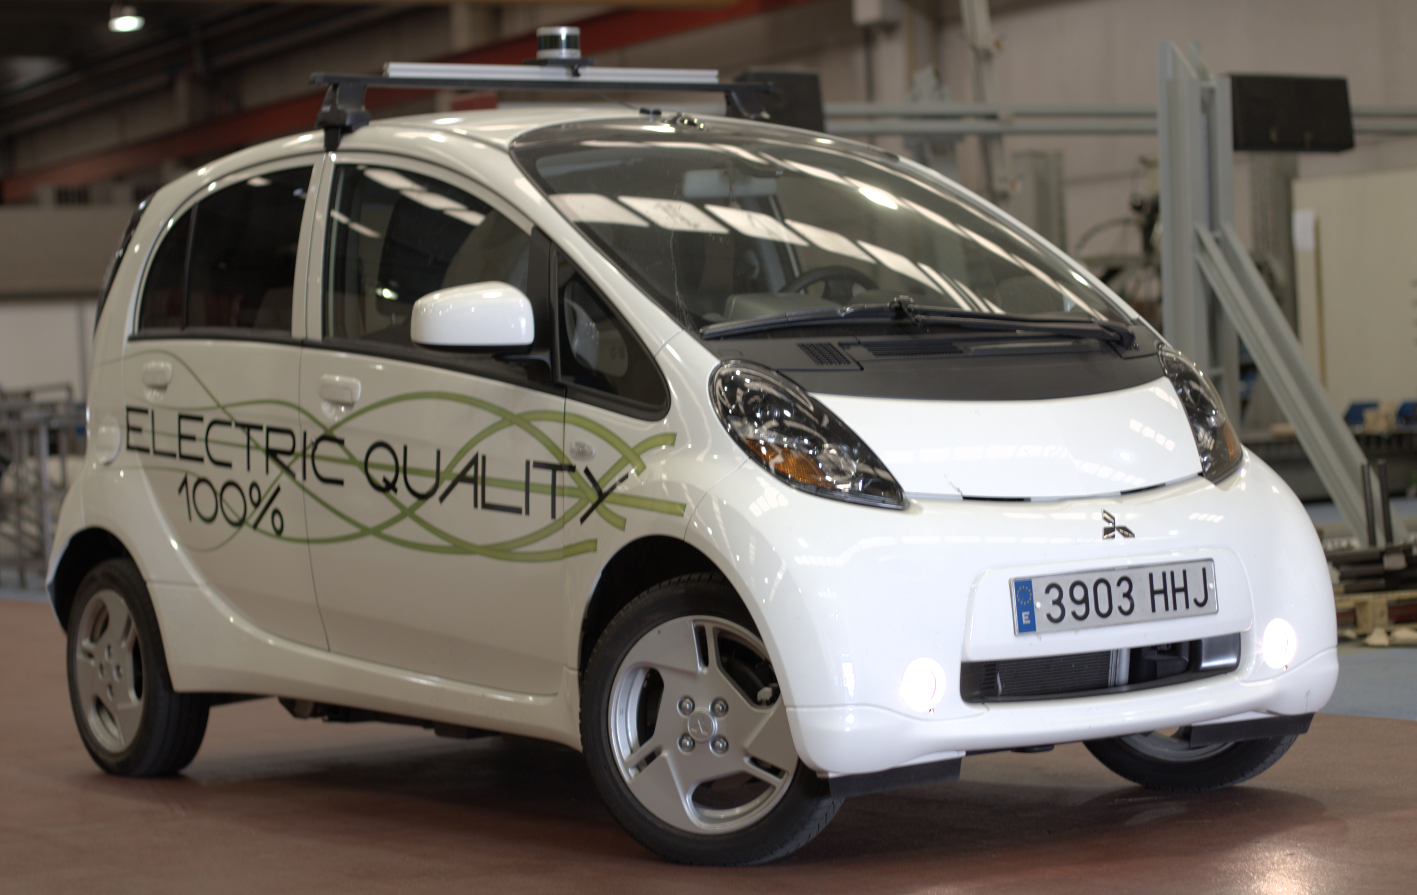
\includegraphics{instrumented-imiev}
	\caption{El vehículo utilizado en los ensayos realizados. Se trata de un Mitsubishi iMiEV instrumentado con un LIDAR anclado en la baca superior, un GPS anclado en el techo, un puerto de acceso directo al Bus CAN y una cámara Microsoft Kinect tras el espejo retrovisor.}
	\label{fig:instrumented-imiev}
\end{figure}

Todos los dispositivos se conectan a un ordenador con sistema operativo GNU/Linux sobre Intel i7-7500U CPU con 16GB de memoria RAM siguiendo el esquema que se muestra en la Figura~\ref{fig:instrumented-imiev-schema}. Al ser éstos dispositivos con capacidades diferentes, se ha optaco por la creación de una aplicación basada en el framework ROS del cual se da una breve visión general en el apéndice~\ref{ch:ros-overview}. A continuación se describen los dispositivos usados y su información generada.

\paragraph{\ac{lidar}}

Un \ac{lidar} es un dispositivo que usa uno o más haces de luz pulsada para el cálculo de la distancia a losobjetos donde éstos impactan.

Nuestro dispositivo en concreto es el modelo VLP-16 de la empresa Velodyne.

Está compuesto por un único haz láser con un movimiento continuo vertical y horizontal capturando información con un vertical de \SI{\pm15}{\degree} distribuído a lo largo de 16 planos (una resolución fija de \SI{2}{\degree}), y un campo horizontal de visión de \SI{360}{\degree} con una resolución dependiente de la velocidad de giro del láser, de \SI{0.1}{\degree} a \SI{0.4}{\degree} para \SI{5}{\Hz} a \SI{20}{\Hz} respectivamente. Estas medidas permiten una captura de 75000 a 300000 puntos del entorno en función de la velocidad de giro a una distancia de hasta \SI{100}{\meter}.

\begin{marginfigure}
	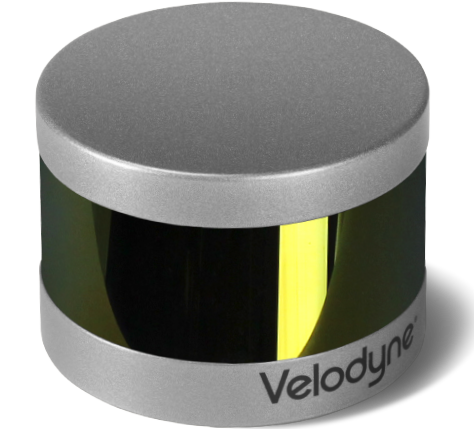
\includegraphics[width=\textwidth]{vlp-16}
	\caption{El \ac{lidar} VLP-16 de Velodyne tiene un FOV horizontal de \SI{360}{\degree} y vertical de \SI{\pm15}{\degree}, permitiendo una captura de todo el entorno circundante a una frecuencia de hasta \SI{20}{\Hz}. Fuente: \url{http://velodynelidar.com/vlp-16.html}.}
	\label{fig:vlp-16}
\end{marginfigure}

El acceso a la información se realiza a través del puerto Ethernet. Para la captura de datos se ha hecho uso de un nodo de \ac{ros} para este tipo de dispositivos \TODO{Explicarlo mejor e indicar el nombre del paquete y su dirección}. Este nodo publica en un topic específico la nube de puntos en coordenadas cartesianas con el eje X definido en el sentido de los \SI{0}{\degree} y el eje Z en sentido ascendente.

El \ac{lidar} se encuentra anclado en la baca del vehículo con el eje X dispuesto en el sentido de conducción y el Z en sentido ascendente. Su posición es centrada en el vehículo y a una altura de \SI{1.75}{\meter}.

\paragraph{\ac{gps}}

El \ac{gps} es una tecnología usada para sincronización de tiempo y posicionamiento 3d (latitud, longitud y altitud) de objetos en el globo terráqueo. Es un dispositivo que funciona en un único sentido, es decir, el receptor recibe la información de los satélites, pero no envía ninguna.

El dispositivo \ac{gps} utilizado para los experimentos ha sido desarrollado en el Laboratorio de Electrónica e Instrumentación del \ac{insia}. Se trata de un dispositivo \ac{gps} con corrección diferencial que genera mensajes \ac{nmea} a una frecuencia de hasta \SI{20}{\Hz}. La posición de la antena receptora estará localizada en el centro del vehículo, justo debajo del \ac{lidar}, situándose de esta forma en el origen de coordenadas del entorno capturado con éste.

\begin{marginfigure}
	\centering
	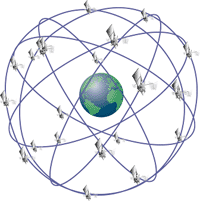
\includegraphics[width=\textwidth]{gps}
	\caption{El \ac{gps} permite el posicionamiento 3d sobre en la tierra gracias a la comunicación unidireccional de satélites situados en órbita. Fuente: Wikimedia Commons.}
	\label{fig:gps}
\end{marginfigure}

De todos los mensajes disponibles, los recuperados son lo de los siguientes tipos:

\begin{itemize}
	\item GGA. Geoposicionamiento del vehículo, el cual será usado para deducir valores no medibles directamente como, por ejemplo, la distancia al siguiente semáforo.
	\item VTG. Velocidad del vehículo, que se usará como el valor real de la velocidad tomada por el vehículo.
\end{itemize}

De la captura de datos se encargará un nodo de ROS \TODO{Explicarlo mejor e indicar el nombre del paquete y su dirección} el cual leerá por el puerto USB la información originada en el \ac{gps}.

\paragraph{Bus CAN}

Un bus es una topología caracterizada por tener un único canal de comunicaciones donde los dispositivos se conectan, vierten la información y la reciben. El bus \acf{can}, o simplemente \ac{can}, es un protocolo de comunicaciones basado en esta topología utilizado, entre otras muchas áreas, la comunicación entre los diferentes dispositivos que componen un vehículo.

El estándar \ac{can} cubre únicamente las dos primeras capas del modelo \ac{osi}\sidenote{
	Las dos primeras capas son la capa física (la conexión el hardware a la red y la transmisión/recepción física de los datos) y la de enlace de datos (direccionamiento físico, detección de errores y control de flujo). Sobre el resto de niveles no existen un estándar definido y por tanto existen multiples protocolos de estas dependiendo del fabricante u organismo que lo implemente.
}, lo cual es suficiente para el acceso a la información del vehículo. Sin embargo, dependiendo del fabricante, los vehículo pueden contar con uno o más buses independientes, con acceso más o menos restringido y con identificadores de mensajes diferentes. Además, el acceso a esta información no suele ser accesible para el público general, por lo que lo normal es realizar una tarea previa de ingeniería inversa para identificar los mensajes correspondientes a los datos que se desean almacenar y su frecuencia.

\begin{marginfigure}
	\centering
	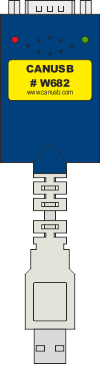
\includegraphics[width=.35\textwidth]{laciwel-canusb}
	\caption{El dispositivo CANBUS de LACIWEL AB permite el acceso a través del protocolo RS 232 por el puerto USB al bus \ac{can}. Fuente: \url{http://www.can232.com/}.}
	\label{fig:laciwel-canusb}
\end{marginfigure}

Del bus se ha recogido numerosa información, tanto para esta tesis como para más proyectos relacionados con ella. Para este experimento, no obstante, se ha utilizados únicamente la velocidad, y no directamente. La razón es que el \ac{can} ofrece ésta como un número entero, por lo que los cambios de velocidad durante los recorridos ocurren de \SI{\pm1}{\km\per\hour}. Esta resolución es insuficiente para los cálculos de la aceleración, por lo que se ha usado para validar la velocidad capturada por el \ac{gps}

El acceso a la información del bus se ha realizado a través del puerto USB. Para ello se ha utilizado el dispositivo CANUSB de la empresa LAWICEL AB, el cual se encarga de la traducción del protocolo CAN a una conexión estándar RS232. La captura de los paquetes se ha realizado a través de un nodo de \ac{ros} desarrollado para esta tesis y descrito brevemente en el apéndice~\nameref{ch:developed-software}.

\paragraph{Cámara}

Para la obtención de algunos valores de indicadores no existentes necesitamos un proceso posterior de análisis sobre el recorrido, asociando las imágenes a los valores recogidos del resto de dispositivos, como posiciones o nube de puntos del entorno. Para ello se ha hecho uso de una cámara para la visualización del recorrido desde el punto de vista del conductor.

La cámara utilizada es un Microsoft Kinect localizada tras el retrovisor interior del vehículo. Dicha cámara está orientada de tal manera que ofrece una visualización de la vía por la que circula el vehículo.

\begin{marginfigure}
	\centering
	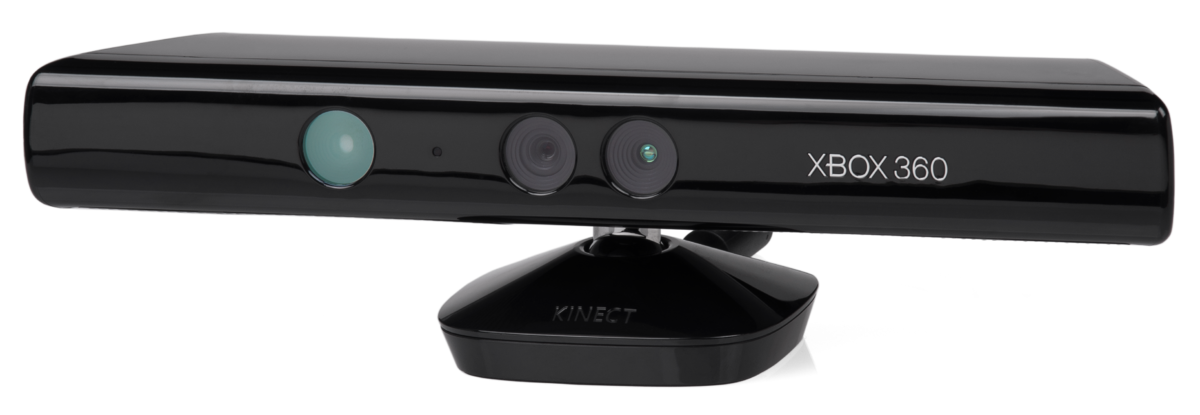
\includegraphics[width=\textwidth]{kinect}
	\caption{La cámara Kinect desarrollada por Microsoft ofrece imágenes a color a una velocidad de \SI{30}{\fps} con una resolución de \SI{640x480}{\px}.}
	\label{fig:kinect}
\end{marginfigure}

Entre otras capacidades, la cámara ofrece captura de imágenes VGA de \SI{640x480}{\px} de resolución y a una frecuencia de \SI{30}{\Hz}. El dispositivo se conecta vía USB y de la captura se encarga un nodo de ROS denominado \textit{freenect}\sidenote{\url{http://wiki.ros.org/freenect\_stack}.} publicando en un topic las imágenes generadas.

\subsection{Selección de rutas}

Para la captura de datos se han propuesto dos rutas, en adelante $R_1$ y $R_2$, consideradas equivalentes. Se tratan de vías en entorno urbano con tramos de entre uno y tres carriles a lo largo de su recorrido y con velocidades máximas establecidas entre los \SI{30}{\km\per\hour} y los \SI{50}{\km\per\hour}. La figura~\ref{fig:proposed-routes} muestra los recorridos en el mapa.

\begin{figure}
	\centering
	\subfloat[]{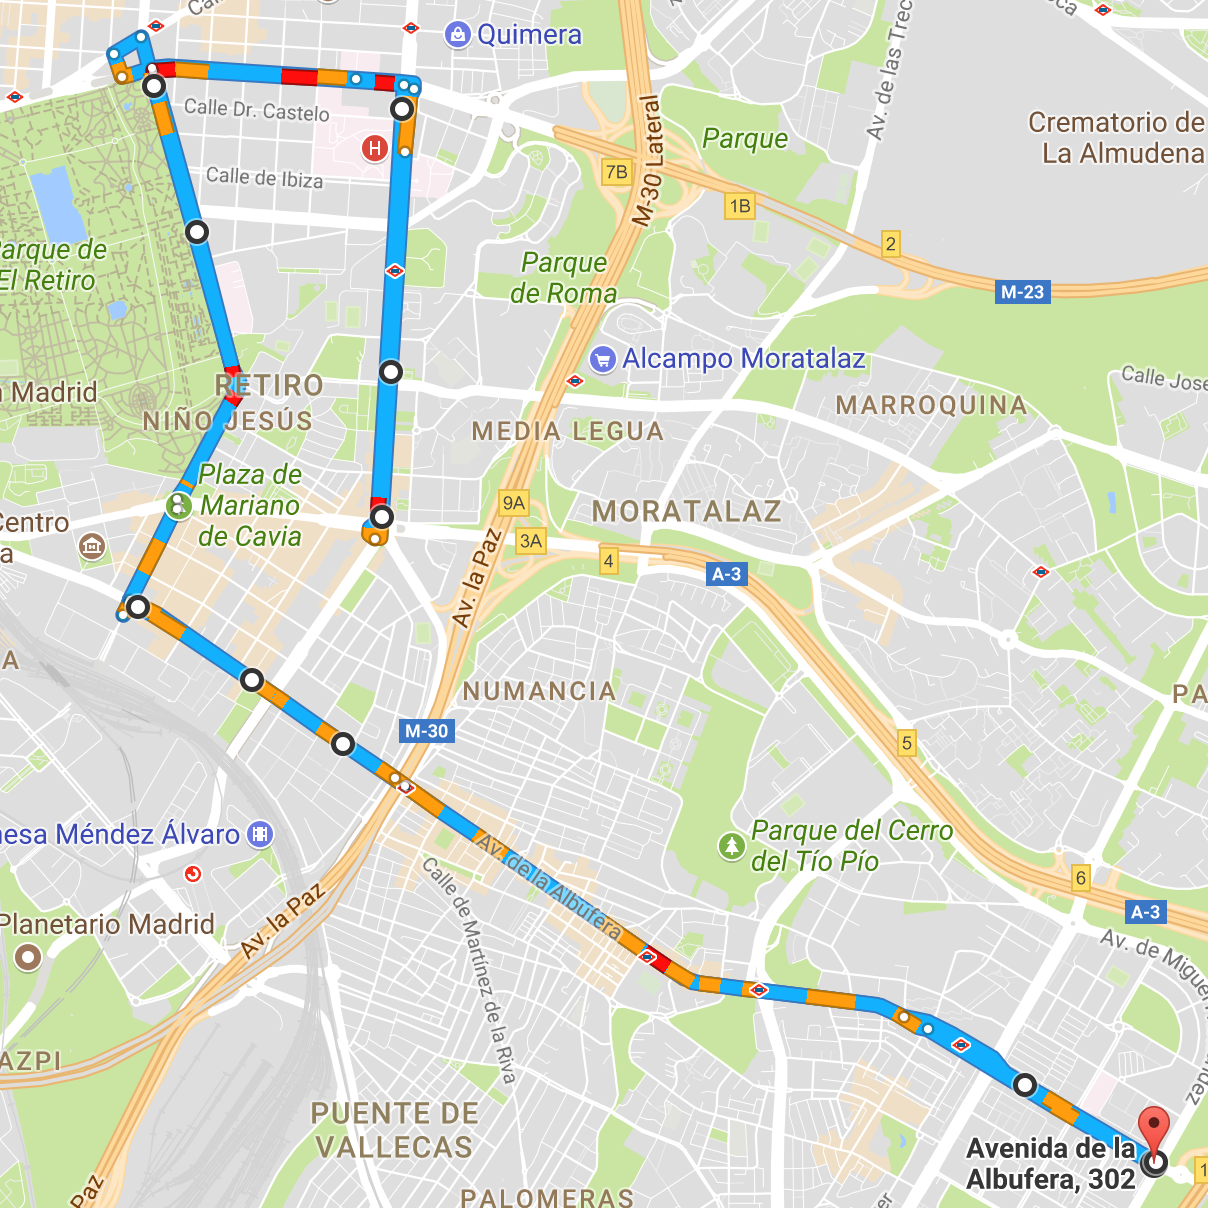
\includegraphics[width=.45\textwidth]{route-1}}\qquad
	\subfloat[]{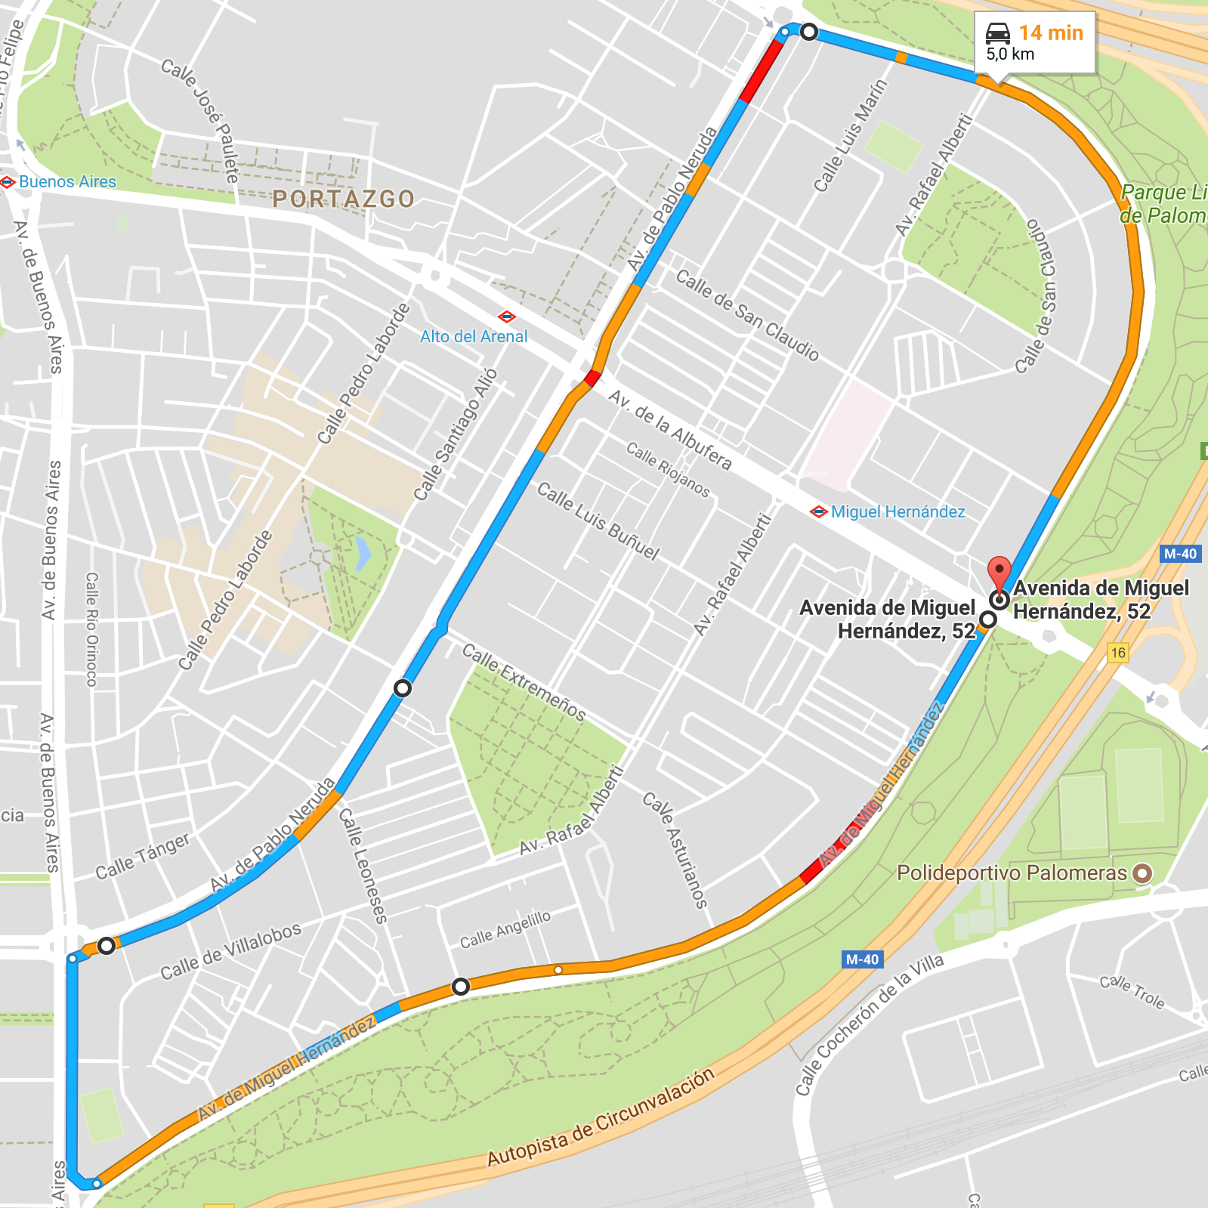
\includegraphics[width=.45\textwidth]{route-2}}
	\caption[Dos recorridos para la captura de datos de conducción]{Los dos recorridos realizados para la captura de datos de conducción, ambos en entorno urbano. (a) $R_1$ tiene una duración estimada de \SI{30}{\minute} y sirve para la captura de los datos de entrenamiento. (b) $R_2$ tiene una duración estimada de \SI{15}{\minute} y sus datos serán utilizdos para los conjuntos de test.}
	\label{fig:proposed-routes}
\end{figure}

$R_1$ tiene una duración de recorrido estimada de \SI{30}{\minute} y se utilizará como fuente de datos destinada al entrenamiento del modelo (conjuntos de entrenamiento y de validación). $R_2$ por su lado tiene un tiempo estimado de recorrido de \SI{15}{\minute} y sus datos tienen el propósito de servir de conjunto de test. Ambas fueron realizadas entre las 11:00am y las 12:00pm en días laborables, permitiendo una circulación con suficientes vehículos para requerir maniobras dependientes del entorno, pero sin demasiados como para impedir la circulación.

\subsection{Selección de sujetos}

Se han elegido un total de tres sujetos para los experimentos. Los tres pertenencen al grupo especificado en los supuestos del capítulo~\nameref{ch:intro}, es decir varones dentro del rango de $35$ a $39$ años.

Los sujetos tienen experiencia de conducción y han realizado el recorrido anteriormente a fin de basar sus comportamientos lo más posible al nivel táctico de conducción\sidenote{
	Dado que los comportamientos de \textit{car-following} y \textit{lane-change} se asocian con el nivel cognitivo táctico, se ha querido reducir el impacto del operador decidiendo durante el experimento hacia dónde o no ir. De esta manera los conductores son librese de realizar el movimiento que deseen y de anticipar maniobras con más libertad.
}.

\TODO{Quizá debería decir algo más?}

\section{Preparación de los datos}

\TODO{Revisar las variables porque han cambiado. Están en el paso 03 de los scripts.}

Tras la captura se ha realizado una secuencia de pasos para dejar los datos preparados para el proceso de entrenamiento de los modelos. El resto de la sección detalla cada uno de éstos.

\subsection{Fusión de sensores}

Como hemos visto anteriormente, cada uno de los dispositivos ofrece sus datos a una tasa de frecuencia diferente (con excepción del bus CAN, en el cual los datos van a frecuencias diferentes).

El primer paso en la preparación de los datos ha sido el de la fusión de estos. Afortunadamente cada uno de los mensajes almacenados que llegan desde nodos de ROS vienen con una marca temporal que podemos suponer sincronizada entre nodos de la misma aplicación. Por ello, la fusión se ha realizado en dos pasos:

\begin{enumerate}
	\item Cálculo del primer elemento a fusionar de cada uno de los conjuntos de datos. Para ello, se han desechado todos los primeros valores hasta encontrar la primera tupla de valores (uno por cada conjunto de datos) donde éstos están más próximos entre si.
	\item Extracción iterativa de las tuplas más aproximadas. Iterativamente, se han ido extrayendo las tuplas más próximas a cada uno de los incrementos de la tasa deseada de sincronización $f$, siempre y cuando se encuentren dentro del intervalo $f \pm \frac{f}{2}$.
\end{enumerate}

Este proceso se ha repetido con cada uno de los conductores para cada uno de los recorridos, dando como resultado seis conjuntos sincronizados con los datos en bruto sincronizados.

\subsection{Extracción de variables no observables directamente}

Existen una serie de variables cuya extracción directa del entorno no es trivial. Ésta es una de las razones por las que se ha capturado con la cámara la visión del conductor en el recorrido.

El proceso de obtenición ha sido manual, obteniendo las marcas temporales de las variables a capturar tras el visionado de las imágenes capturadas por la cámara. Estas variables son las siguientes:

\paragraph{Cambio de carril}

Se han identificado los cambios de carril, siendo estos marcados como $+1$ si es un cambio hacia la izquierda o $-1$ si es un cambio a la derecha, y por tanto, todos aquellos momentos en los que no hay cambio de carril se marcan tendrán un valor de $0$. Las marcas temporales de los cambios son aquellas desde el comienzo de la maniobra del cambio de carril hasta que el vehículo ha llegado a la mitad del cambio.

\paragraph{Velocidad máxima de la vía}

Se han añadido las velocidades máximas de las vías indicando las marcas temporales en las que el conductor entra o sale de cada uno de los tramos.

\paragraph{Distancia y estado de semáforos}

La distancia al semáforo ha sido obtenida a partir de la distancia euclídea entre la geoposición del origen de coordenadas y la geoposición del semáforo, por lo que es esperable cierto márgen de error. Los estados se han extraído directamente del visionado de las imágenes, tomando este los valores $g$, $y$ y $r$ dependiendo de si el semáforo se encuentra en verde, ámbar o rojo.

\paragraph{Distancia a recorrer en carriles}

Al igual que con la distancia a los semáforos, ésta se ha calculado a partir de la distancia euclídea de la geoposición del origen de coordenadas a los puntos a partir de los cuales no se puede continuar por el recorrido especificado.

Las distancias obtenidas se corresponden al carril izquiero, al actual y al derecho.

\paragraph{Distancia al obstáculo más cercano}

Para el cálculo de esta variable, se ha procedido a capturar una región de interés de cada una de las nubes de puntos dentro de la cual identificar los posibles obstáculos existentes. Por la posición del lidar se ha decidido que ésta está acotada entre los intervalos $(0.35, 35)$, $(-1, 1)$ y $(-1.5, 0.5)$ para los ejex X, Y y Z respectivamente.

Posteriormente, para la nube de puntos resultante se ha realizado un proceso de clusterización aplicando el algoritmo DBSCAN\sidenote{
	DBSCAN~\cite{ester1996density} es un algoritmo de clusterización que identifica un número variable de conjuntos en un espació $n$-dimensional.
	
	Funciona a partir de la agregación de puntos en función de sus parámetros $\epsilon$ y $\mu$. $\epsilon$ es la distancia mínima a la que se deben encontrar dos puntos para considerarse pertenecientes al mismo clúster mientras que $\mu$ determina el número mínimo de puntos que debe tener un clúster para ser considerado como tal.
} con parámetros $\epsilon = 0.5$ y $\mu = 3$. Este proceso identifica un número variable de clústers, tras el cual nos hemos quedado con el más cercando al vehículo.

Posteriormente y de forma manual, se ha realizado el recorrido mostrando las nubes de puntos correspondientes a las capturas superponiendo el centroide para eliminar los de aquellos frames que se corresponden con errores. De los restantes se ha calculado una distancia euclídea al origen de coordenadas.

\subsection{Curación de datos}

Tras obtener todas las variables principales, ya sean obtenidas directamente de los sensores del coche o a través de un proceso manual vamos a generar los conjuntos de datos para los comportamientos longitudinal y de cambio de carril. La tabla~\ref{tbl:main-variables} describe qué variables son usadas en qué conjunto de datos.

\begin{table}[t]
	\caption[Resúmen de información extraída del vehículo instrumentado]{Valores capturados por el vehículo instrumentado y sus dominios. Los valores de 0, 1 y 2 se corresponden con los cambios de carril, siendo 0 cambio a la izquierda, 1 no cambio y 2 a la derecha.}
	\label{tbl:main-variables}
	\begin{tabular}{lll}
		\toprule
		Variable & Longitudinal & Cambio de carril \\
		\midrule
		Acceleration      & \yep & \yep \\
		Distance +1       & \nop & \yep \\
		Distance 0        & \nop & \yep \\
		Distance -1       & \nop & \yep \\
		Lane change       & \nop & \yep \\
		Leader distance   & \yep & \nop \\
		Next TLS distance & \yep & \yep \\
		Next TLS status   & \yep & \yep \\
		Nube de puntos    & \nop & \yep \\
		Relative speed    & \yep & \yep \\
		Speed to leader   & \yep & \nop \\
		\bottomrule
	\end{tabular}
\end{table}

\subsection{Generación artificial de datos}

Los problemas con alta variabilidad de sus entradas suelen ser complejos y requerir de conjuntos de datos de tamaños bastante grandes para poder identificar patrones, como lo son por ejemplo los problemas de reconocimiento de imágenes.

En nuestro caso, el modelo de cambio de carril tiene como entrada una nube de puntos, la cual representa en un espacio de 3 dimensiones un conjunto muy limitado de puntos, con la dificultad añadida de que el LIDAR tiene de base un error de \SI{3}{\cm}. Como el espacio sobre el que trabajar es tan complejo, se requerirían modelos con muchos parámetros, pero al disponer de pocos ejemplos, podríamos caer muy fácilmente en problemas de \textit{over-fitting}.

Por ello, se ha optado por realizar un proceso de generación de datos artificiales a partir de los datos existentes. De esta manera, ayudaremos al modelo a entrenar con casos similares y que de esta manera generalice mejor. La aumentación se ha realizado sobre los datos recogidos en la ruta $R_1$, ya que es la que nos proporciona la información para entrenar el modelo y es por tanto en el único conjunto que cobra sentido este proceso. Concretamente hemos hecho uso de dos técnicas, primero un \textit{mirroring} sobre todas las filas del conjunto y diez aplicaciones de la técnica \textit{shaking} sobre el nuevo conjunto con los datos originales y simétricos.

La aplicación de estas técnicas requiere además que las nuevas porciones de datos generadas mantengan una coherencia temporal. Por tanto, aunque pertenezcan al mismo conjuntos de datos, cada uno se mantiene en una secuencia independiente.

A continuación se pasan a describir los procesos de generación de datos artificials introducidos previamente.

\paragraph{mirroring}

Se parte de la suposición de que los procesos cognitivos que producen determinados comportamientos (en nuestro caso, el cambio de carril) son los mismos independientemente de un cambio a la izquierda o hacia la derecha\sidenote{
	Es una suposición que en estudios sucesivos se puede tratar de refutar. Sin embargo, en el estadio actual de la investigación, nos parece razonable asumir que los procesos cognitivos en ambas situaciones son equivalentes.
}.

Por tanto, para cada fila generaremos una nueva nube de puntos a partir de una simetría respecto al plano XY (recordemos que el eje X determina el sentido del movimiento del vehículo). De esta manera, modificando las variables pertinentes\sidenote{
	 Es decir, invirtiendo los cambios de carril y la distancia recorrible en carriles izquierdo y derecho.
}, de cada ejemplo obtenemos uno nuevo. En la figura~\ref{fig:mirroring-example} se ilustra un ejemplo de este proceso sobre una nube de puntos arbitraria dentro del conjunto de ejemplos.

\begin{figure}
	\centering
	\subfloat[]{\missingfigure[figwidth=.43\textwidth]{Nube de puntos}}\qquad
	\subfloat[]{\missingfigure[figwidth=.43\textwidth]{Nube de puntos tras mirroring}}
	\caption[Ejemplo de la técnica de \textit{mirroring}]{Un ejemplo de una nube de puntos (a) original, y (b) tras aplicarle el proceso de mirroring. Para cada fila, tras un proceso de mirroring y una inversión de las variables simétricas en función de la conducción (cambio de carril y distancia recorrible) se genera una nueva fila válida para el conjunto de datos.}
	\label{fig:mirroring-example}
\end{figure}

La principal ventaja de esta aproximación es que es posible doblar el tamaño del conjunto de datos sin afectar añadir más ruido al existente en los mismos.

\paragraph{shaking}

Esta técnica, a diferencia del \textit{mirroring} sí puede llegar a tener impacto en la precisión de los datos. Partiendo de una nube de puntos original\sidenote{
	Debido a que la aplicación iterativa de este proceso sobre la misma nube de puntos acumula los errores entre iteraciones haciéndola ininteligible.
}, se aplica un desplazamiento aleatorio $(\delta x, \delta y, \delta z)$ sobre cada punto tal y como se describe en~\cite{EL PAPER CUANDO NOS LO PUBLIQUEN}. La figura~\ref{fig:shaking-example} ilustra dos procesos de shaking con diferentes desplazamientos sobre la nube original mostrada en la figura~\ref{fig:mirroring-example}

\begin{figure}
	\centering
	\subfloat[]{\missingfigure[figwidth=.43\textwidth]{Nube de puntos con shaking de 0.05}}\qquad
	\subfloat[]{\missingfigure[figwidth=.43\textwidth]{Nube de puntos con shaking de 0.1}}
	\caption[Ejemplo de la técnica de \textit{shaking}]{Un ejemplo de dos nubes de puntos tras pasar el proceso de shaking con un desplazamiento $(\delta x, \delta y, \delta z)$ de (a) $(0.05, 0.05, 0.05)$ y de (b) $(0.2, 0.2, 0.2)$ sobre la nube de puntos original. Para cada fila, tras un proceso de shaking disponemos de una nueva fila ligeramente diferente de la original, añadiendo ruido y, presumiblemente, generalización al modelo tras el entrenamiento.}
	\label{fig:shaking-example}
\end{figure}

Las especificaciones técnicas del LIDAR usado en los experimentos garantizan un error por debajo de los \SI{3}{\cm} de radio, por lo que un desplazamiento aleatorio para cada punto menor o igual que este valor no añadiría más ruido del existente. Sin embargo, en el experimento se ha optado sin embargo por aplicar un desplazamiento de $\delta x = \delta y = \delta z = 0.05m$ en cada eje, ligeramente superior al proporcionado por el lidar. De esta forma se pretende la incorporación de ruido sobre el entorno original para aumentar la capacidad de generalización del modelo\sidenote{
	La intuición de este proceso
}.

\subsection{Representación de los datos}

Las secuencias de las que se compone el conjunto de datos están compuestas, aparte de variables numéricas, de una representación del entorno del vehículo como nube de puntos. Los límites técnicos y la representación en sí implican dos problemas principales:

\begin{enumerate}
	\item Los modelos que utilizamos en esta tesis se basan en un número fijo de entradas, y la nube de puntos contiene un número variable de éstos, dependiendo del número de obstáculos y su distancia al origen.
	\item La nube de puntos se origina a través de un dispositivo mecánico que funciona con coordenadas esféricas a una resoluciones horizontal de \SI{0.2}{\degree}\sidenote{
		Funcionando a \SI{10}{\hertz}.
	} y vertical de \SI{2}{\degree}. Esto implica que la superficie del sector circular que no se cubre a largas distancias sea muy extenso, por lo que el espacio según nos alejamos del origen va siendo cada vez más diperso.
\end{enumerate}

Para el primer caso, se ha optado por representar el entorno como un mapa de profundidad, ilustrado en la Figura~\ref{fig:deepmap-example}. Un mapa de profundidad representa el entorno como una imagen de un sólo canal donde cada píxel representa la distancia a un sector esférico del espacio original.

\begin{figure*}
	\centering
	
\includegraphics{deepness-map}
	\caption[Ejemplo de un mapa de profundidad]{Un ejemplo del mapa de profundidad asociado a la nube de puntos original.}
	\label{fig:deepmap-example}
\end{figure*}


Dado que el LIDAR describe el entorno de manera discreta con valores constantes de elevación y azimuth, se puede definir una biyección entre el conjunto de puntos original y los píxeles del mapa de profundidad, por lo que la información disponible en ambas es equivalente. Sin embargo, en nuestro caso no necesitamos una representación tan fiel del entorno porque:

\begin{itemize}
	\item La resolución horizontal produce un mapa de profundidad de $1800$ columnas. Esta resolución es extremadamente grande, y requeriría el uso de modelos con muchos parámetros, pudiendo caer fácilmente en un problema de \textit{over-fitting}.
	\item La apertura vertical del LIDAR genera puntos en planos que no son relevantes para el problema. Esto es, planos muy bajos que impactan en el vehículo o muy altos que no impactan con el entorno considerado de interés.
\end{itemize}

Por estas razones, los mapas de profundidad se generarán de una manera más compacta, usando una resolución horizontal de \SI{1}{\degree} y los seis canales que van desde los \SI{-7}{\degree} hasta los \SI{3}{\degree}, lo que nos da un mapa de profundidad con una resolución de $6 \times 360$ con un canal representando la distancia al punto de impacto más cercano contenido en el sector esférico que representa cada posición del mapa\sidenote{
	\TODO{Determinar si tiene sentido explicar aquí el proceso de generación del mapa de profundidad (el algoritmo).}
}.

Para el segundo caso, se ha definido un radio de interés de \SI{25}{\meter}, ya que se ha considerado para el proceso de cambio de carril como un entorno lo suficientemente amplio para determinad un cambio de carril.

Con estos datos, los mapas de profundidad serán normalizados al intervalo $[0, 1] \in \mathbb{R}$ invertido, esto es, los valores mas cercandos al vehículo serán más próximos a 1 mientras que los valores más alejados estarán más próximos a 0.

\subsection{Descripción de los datasets}

Hasta este punto disponemos de un conjunto relativamente grande de secuencias ordenadas en el tiempo, de tal manera que dentro de cada secuencia cada una de las filas está situada \SI{0.1}{\second} más adelante en el tiempo que la anterior. La tabla~\ref{tbl:data-of-datasets}

\begin{table*}[t]
	\caption[Resúmen de información extraída del vehículo instrumentado][1.5em]{Valores capturados por el vehículo instrumentado y sus dominios. Los valores de 0, 1 y 2 se corresponden con los cambios de carril, siendo 0 cambio a la izquierda, 1 no cambio y 2 a la derecha.}
	\label{tbl:data-of-datasets}
	\begin{tabular}{lll}
		\toprule
		Variable & Descripción & Dominio \\
		\midrule
		LiDAR & Coordenadas de todos los puntos capturados por el dispositivo. & $[-200m, 200m] \subset \mathbb{R}$ \\
		\bottomrule
	\end{tabular}
\end{table*}

Para entrenar los modelos correspondientes a cada una de las hipótesis, se generarán los siguientes datasets:

\begin{itemize}
	\item Entrenamiento y test de modelo longitudinal para todos los sujetos en general.
	\item Entrenamiento y test de modelo longitudinal para cada uno de los sujetos de estudio por separado.
	\item Entrenamiento y test de modelo de cambio de carril para todos los sujetos en general.
	\item Entrenamiento y test de modelo de cambio de carril para cada uno de los sujetos de estudio por separado.
\end{itemize}

Como nuestros modelos se basan en un esquema \textit{feed-forward}, existe el inconveniente de que para ellos es imposible mantener una memoria del orden en el que se están sucediendo las entradas.

\begin{figure*}
	\centering
	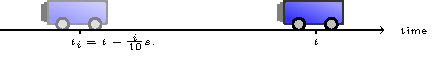
\includegraphics{explanation-of-data-frequency}
	\caption[Momento $t_i$en el conjunto de datos]{Un momento $t_i$ se define como el estado en el que se encontraba el vehículo en $t - \frac{i}{10}s$. Por tanto, $t_0$ es el momeno actual.}
	\label{fig:moments-illustration}
\end{figure*}

En el caso del modelo de longitudinal es útil para obtener información acerca de la aceleración del vehículo o de la velocidad con la que nos aproximamos al vehículo delantero, pero afortunadamente estos datos son cuantitativos y han sido calculados previamente a partir de las diferencias de las velocidades y de las distancias respectivamente. En el caso del modelo de cambio de carril la solución no es tan sencilla.

En cada una de las filas poseemos un mapa de profundidad que describe el entorno, por lo que al modelo le alimentaríamos únicamente con la situación en un instante $t$ de tiempo. Esto no ayuda al modelo a descubrir patrones temporales como la velocidad o la aceleración puesto que no tiene información de eventos anteriores. Para solventar esta limitación, los conjuntos de datos serán transformados para que se alimenten con una ventana temporal de parámetros de entrada.

Comenzaremos definiendo el \textit{momento} $t_i$ como aquel ejemplo situado a $t - \frac{i}{10}s$ en el pasado (ver Figura~\ref{fig:moments-illustration}). Los momentos que se tendrán en cuenta en los datasets finales serán $t_0$, $t_5$, $t_10$, correspondientes al momento actual y \SI{0.5}{\second}, \SI{1}{\second} y \SI{2}{\second} previos respectivamente. Estos valores no son arbitrarios, sino que se han elegido de acuerdo a los experimentos realizados en~\cite{EL PAPER CUANDO NOS LO PUBLIQUEN}\sidenote{
	Dichos experimentos se corresponden con el proceso de ejecución de cambio de carril, donde se asume que la maniobra involucra al córtex visual y al córtex prefrontal. Estos procesos cognitivos tienen un tiempo de respuesta de entre \SI{0.2}{\second}, \SI{1.2}{\second}~\cite{buzsaki2012temporal}, por lo que es comprensible que la ventana temporal elegida sea aceptable. Además, al incluir tres momentos temporales, es posible que el modelo reconozca una intuición de la velocidad, la aceleración e incluso el \textit{jerk} a partir de imágenes estáticas. 
}.

Tras este ajuste, los conjuntos de datos están finalizados. Sus propiedades quedan descritas en la Tabla~\ref{tbl:datasets-description}.

\begin{table}[t]
	\caption[Descripción de los conjuntos de datos]{Descripción de los conjuntos de datos para el entrenamiento de los modelos.}
	\label{tbl:datasets-description}
	\begin{tabular}{lllll}
		\toprule
		Nombre & Entradas & Salidas & Tamaño (training) & Tamaño (test) \\
		\midrule
		$LT_{S_1}$ & \yep & \yep & \yep & \\
		$LT_{S_2}$ & \nop & \yep & \yep & \\
		$LT_{S_3}$ & \nop & \yep & \yep & \\
		$LT_{S_A}$ & \nop & \yep & \yep & \\
		$CT_{S_1}$ & \nop & \yep & \yep & \\
	    $CT_{S_2}$ & \yep & \nop & \yep & \\
		$CT_{S_3}$ & \yep & \yep & \yep & \\
		$CT_{S_A}$ & \yep & \yep & \yep & \\
		\bottomrule
	\end{tabular}
\end{table}

\section{Entrenamiento de modelos}

Para cada uno de los submodelos se han probado dos aproximaciones diferentes para comparar sus desempeños en las tareas por separado. Concretamente se han utilizado \acp{fcs} y \acp{mlp} para modelar el comportamiento longitudinal y \acp{mlp} y \acp{cnn} para modelar el comportamiento en cambio de carril.

El resto de la sección describe el modelo que componen estos dos modelos de comportamiento y el proceso de entrenamiento de los mismos.

\subsection{Perspectiva general}

Para el diseño y ajuste del modelo de conductor se ha decidido separar los dos comportamientos principales que componen el nivel cognitivo táctico, estos son, el modelo longitudinal y el modelo de cambio de carril.

La idea es diseñar el \ac{dvu} como un agente con un modelo de comportamiento que actúe sobre (i) la aceleración/deceleración, y (b) la decisión y ejecución del cambio de carril, ambos a partir de los estímulos recibidos del exterior. Estos estímulos serán replicados en el simulador para que los agentes con los modelos entrenados con estímulos del mundo real reciban estímulos similares en estos entornos.

Internamente, el modelo estará separado en los dos modelos básicos, el modelo longitudinal y el de cambio de carril. En la Figura~\ref{fig:overall-driver-model-schema} se describe el modelo, las entradas y salidas y el flujo de datos entre componentes.

\begin{figure*}
	\centering
	\missingfigure[figwidth=5cm]{Esquema general del modelo de conductor}
	\caption[Esquema general del modelo de conductor planteado]{Esquema general del modelo de conductor planteado en la tesis. En éste se puede ver cómo se distribuyen los estímulos de entrada entre los diferentes componentes del modelo y las salidas del sistema, que irán conectadas a los actuadores pertinentes.}
	\label{fig:overall-driver-model-schema}
\end{figure*}

\TODO{No se me ocurre qué más añadir aquí.}

Para los entrenamientos de los modelos se ha utilizado una máquina con procesador Intel\textregistered Core\texttrademark i7-6700K a \SI{4.00}{\giga\Hz} y \SI{16}{\gibi\byte} de memoria. El sistema operativo utilizado ha sido un Debian GNU/Linux versión 9.4.

\subsection{Comportamiento longitudinal}

El comportamiento longitudinal es un problema de regresión sobre cómo ha de comportarse la aceleración del \ac{dvu} en función de la información existente alrededor.

Como este problema en concreto no parece excesivamente complejo, se han seleccionado un subconjunto de las variables capturadas para determinar el comportamiento de la aceleración, y ésta se inferirá a través de dos modelos:

\begin{enumerate}
	\item \ac{mlp}. \TODO{No se me ocurre qué escribir para justificarlo.}
	\item \ac{fcs}. La formulación de este problema se ajusta muy bien al funcionamiento de estos modelos, donde en función de las entradas y de acuerdo a una serie de reglas, el controlador toma una decisión para la salida. Además, los \ac{fcs} tienen la ventaja de que se puede explicar cómo funcionan, cosa que no es posible para un \ac{mlp} con una o más capas ocultas.
\end{enumerate}

Ambos modelos se entrenaran ajustando sus parámetros con un procedimiento basado en el descenso del gradiente denominado ADAM~\cite{kingma2014adam}. Su aplicación a los \ac{mlp} es directa, pero para \acp{fcs} es necesaria una representación que permita el uso de este método para su optimización. Esta representación es una de las aportaciones de esta tesis y se se explicará a lo largo de la sección.

\paragraph{Modelo \ac{fcs}}

Se han tomado las siguientes decisiones de diseño para facilitar el desarrorrollo del controlador. Aún así, éstas son fácilmente modificables:

\begin{itemize}
	\item Las funciones de pertenencia serán, o bien una línea descendente en el caso del primer conjunto difuso de una partición, una línea ascendente en el caso del último o trapecios en el caso del resto.
	\item Las $t$-norma y $t$-conorma serán el máximo y el mínimo respectivamente. La $t$-norma se usará como operador asociado al AND lógico y a la implicación, mientras que la $t$-conorma se usará como operador asociado al OR lógico y a la acumulación.
	\item El controlador será de tipo Sugeno, representando las funciones de salida como conjuntos difusos de tipo singletón y con función de defuzzificación CoGS\sidenote{
		$CoGS = \sum_{i=1}^n w_i \cdot o_i$
	}.
	\item El tamaño de las particiones difusas será dado de antemano.
	\item El controlador tendrá una única variable de salida.
\end{itemize}

Como vimos en la sección~\ref{ss:fcs} del capítulo~\nameref{ch:sota-ci}, un \ac{fcs} se compone de cuatro bloques diferenciados: la fuzzificación, el bloque de reglas, la inferencia y la defuzzificación. De éstos bloques, el proceso manual de ajuste se resume siempre\sidenote{
	Por supuesto implica más ajustes como la elección de las funciones de fuzzificación, las $t$-normas y $t$-conormas, de la función de defuzzificación, pero estas operaciones no tienen tanto impacto en el desempeño del controlador como las particiones difusas y las reglas.
} en dos pasos:

\begin{enumerate}
	\item Elección de las particiones difusas de las variables lingüísticas.
	\item Definición de las reglas difusas.
\end{enumerate}

Las soluciones de ajuste que existen en la literatura suelen funcionar ajustando automáticamente uno de los dos puntos manteniendo constante el otro (e.g. ajustar las particiones manteniendo fijas las reglas). Nosotros representaremos el controlador como un grafo computacional de manera que sus gradientes sean sencillos de ajustar\sidenote{
	Como veremos más adelante, el tiempo de ajuste con esta representación es muy rápido, lo que abre la posibilidad de desarrollar un algoritmo que incluya este para el ajuste de los metaparámetrosdel controlador, como por ejemplo los tamaños de las particiones.
}.

\newthought{El bloque de fuzzificación} está compuesto por variables lingüísticas, compuestas por conjuntos difusos definidos por funciones de pertenencia. Estas funciones de pertenencia son las que definen las particiones y son las que contienen los parámetros ajustables. Nosotros usaremos la línea ascendente, la línea descendente y el trapecio.

\begin{marginfigure}
	\missingfigure[figwidth=\textwidth]{Line desc}
	\caption{Función de pertenencia linea descendente definida por $(a, \delta b)$.}
	\label{fig:line-asc}
\end{marginfigure}

\begin{marginfigure}
	\missingfigure[figwidth=\textwidth]{Line asc}
	\caption{Función de pertenencia linea descendente definida por $(a, \delta b)$.}
	\label{fig:line-desc}
\end{marginfigure}

\begin{marginfigure}
	\missingfigure[figwidth=\textwidth]{Trapz}
	\caption{Función de pertenencia linea descendente definida por $(a, \delta b, \delta c, \delta d)$.}
	\label{fig:trapz}
\end{marginfigure}

\begin{figure}
	\centering
	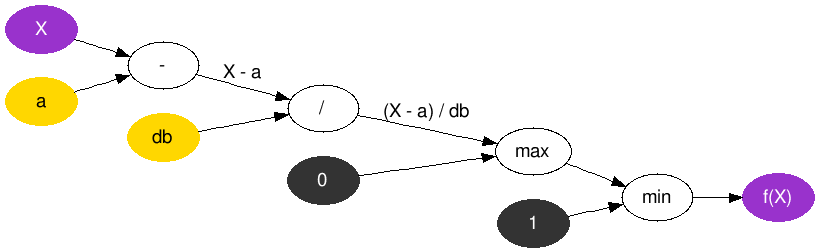
\includegraphics{slope-asc-graph}
	\caption[Grafo computacional de la función de pertenencia para la línea ascendente]{Ilustración del grafo computacional para la función de pertenencia línea ascendente. La fórmula que describe es $\mu(x) = \min(\max(\frac{x - a}{\delta b}, 0), 1)$, quedando acotada $\mu(x)$ en el intervalo $[0, 1] \in \mathbb{R}$. El grafo computacional para la línea descendente es similar y se corresponde con la fórmula $\mu(x) = \min(\max(\frac{a - x}{\delta b + 1}, 0), 1)$.}
	\label{fig:slope-asc-grap}
\end{figure}

Las líneas \textbf{ascendente} y \textbf{descendente} tienen una forma parecida. El grafo asociado a la fórmula de la línea descendente se muestra en la figura~\ref{fig:slope-asc-grap}, que es la que se correspondería con el último conjunto de una partición difusa. Como se puede ver, las variables ajustables son $a$ y $\delta a$. Estas definen el intervalo $(a, a + \delta b) \in \mathbb{R}$ donde los valores $f(X)$ ascienden de $0$ a $1$ (o descienden de $1$ a $0$ en el caso de la recta ascendente).

El \textbf{trapecio} se define a partir de los parámetros $(a, \delta b, \delta c, \delta d) \in \mathbb{R}$, que definen los intervalos $I_1 = (a, a + \delta b)$, $I_1 = (a + \delta b, a + \delta b + \delta c)$ y $I_3 = (a + \delta b + \delta c, a + \delta b + \delta c + \delta d)$. $I_1$ es el intervalo donde la función de pertenencia aumenta su valor de $0$ a $1$, $I_2$ el intervalo superior del trapecio donde la función vale $1$ e $I_3$ donde la función comienza a descender su valor de $1$ a $0$. El grafo asociado a esta función se ilustra en la figura~\ref{fig:trap-graph}

\begin{figure}
	\centering
	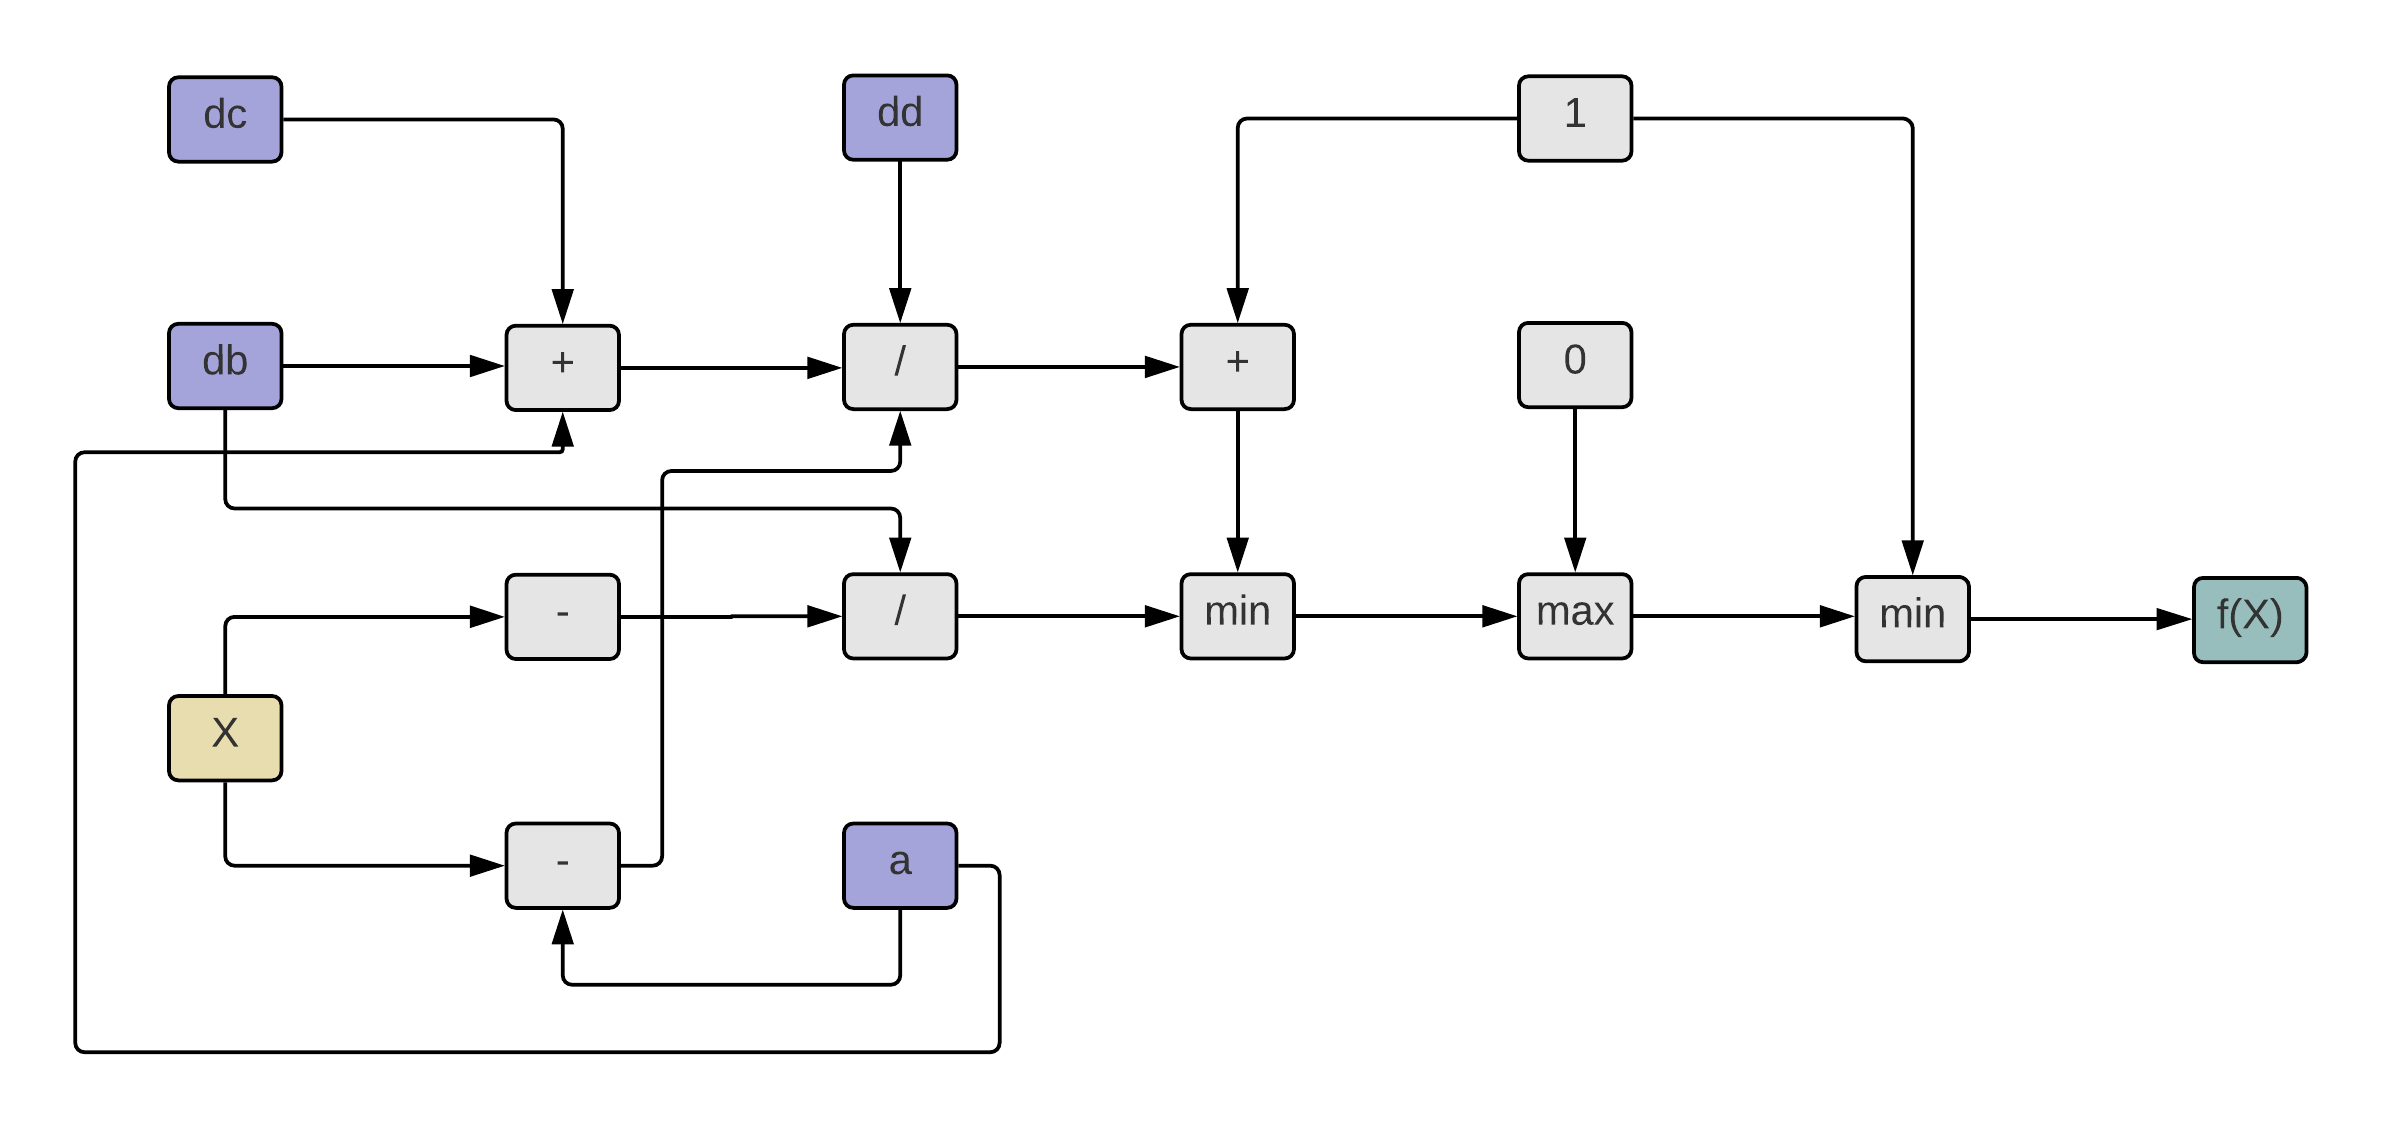
\includegraphics{trap-graph}
	\caption[Grafo computacional de la función de pertenencia para el trapecio]{Ilustración del grafo computacional para la función de pertenencia trapezoidal. La fórmula que describe es $\mu(x) = \min(\max(\min(\mu_{L_{asc}}, \mu_{L_{desc}}), 0), 1)$, esto es, una línea ascendente y otra descendente, estando ambas acotadas en el intervalo $[0, 1] \in \mathbb{R}$.}
	\label{fig:trap-grap}
\end{figure}

Sabiendo los grafos computacionales de cada una de las funciones de pertenencia, ya podemos definir el grafo asociado a la partición difusa de una variable lingüística. Suponiento que la variable $V$ está dividida en $n$ conjuntos difusos, la partición de ésta estará compuesta de:

\begin{itemize}
	\item Un primer conjunto definido como una pendiente descendente.
	\item $n - 2$ conjuntos definidos por una función de pertenencia de tipo trapezoidal.
	\item Un último conjunto definido como una pendiente ascendente.
\end{itemize}

Este grafo tiene que definir una serie de variables para que nuestro algoritmo de entrenamiento las ajuste correctamente. Estas variables están directamente relacionadas con los parámetros de las funciones de pertenencia descritas anteriormente. Hemos decidido por tanto establecer estas variables como los espacios existentes entre los puntos caracteríscos de las funciones. En la figura~\ref{fig:fuzzification-graph-vars} se puede observar de qué manera están relacionadas las variables de desplazamiento y los parámetros de las funciones de pertenencia.

\begin{figure}
	\centering
	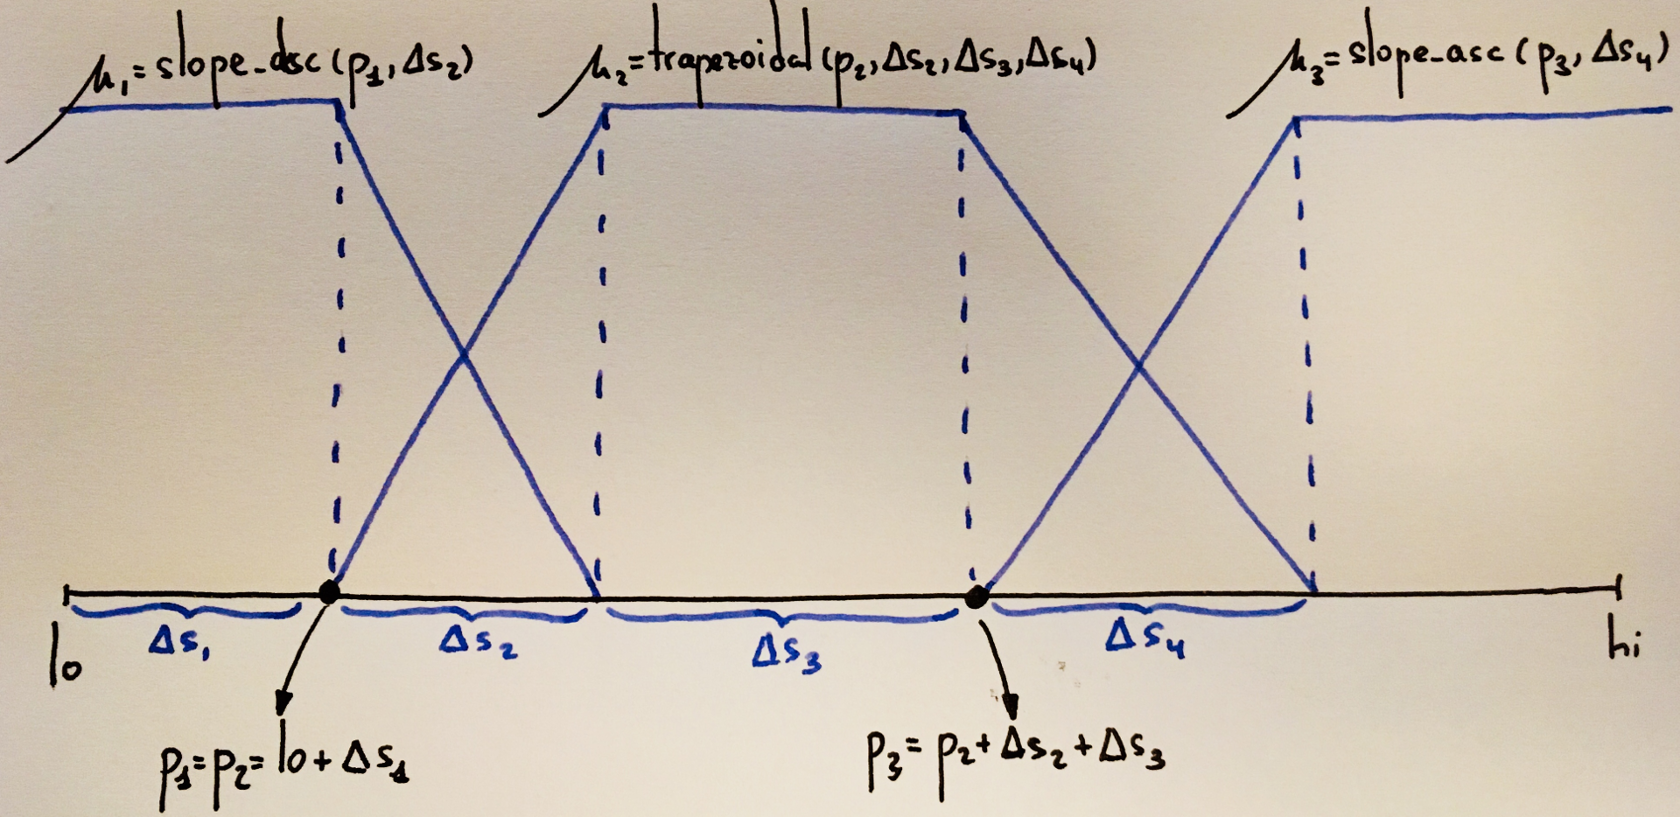
\includegraphics{fuzzification-graph-vars}
	\caption[Representación de una partición difusa para su ajuste]{Ilustración de una partición difusa para una variable lingüística con $n = 3$ conjuntos difusos en el dominio $[l, h]$. Al ser $n = 3$, la partición queda definida como un punto de origen $l$ y $2(n - 1)$ variables correspondientes a desplazamientos consecutivos, los cuales son los que definen los parámetros de las funciones de pertenencia de cada uno de los conjuntos difusos. A partir de este punto, los grafos computacionales son más complejos y su ilustración no aporta nada, por lo que los conceptos se ilustrarán de forma diferente.}
	\label{fig:fuzzification-graph-vars}
\end{figure}

Al estar definidas de esta manera, logramos (i) que la suma de todas las pertenencias en cada punto del eje $X$ es $1$ y (ii) que cada pequeña variación del gradiente de una de las variables tiene el potencial de provocar una variación en el resto de variables.

Por último, un controlador difuso define un número de variables de entrada. Nuestro grafo de fuzzificación estará definido de tal manera que para una matriz de entrada $m \times l$, siendo $m$ cada tupla de valores a inferir y $l$ cada una de las variables lingüísticas, generará una matriz de la forma $m \times \sum_{i=1}^l \left\vert{l_i}\right\vert$, siendo $\left\vert{S}\right\vert$ el número de conjuntos difusos que contiene la variable linguística $l_i$ (Figura~\ref{fuzzification-graph})

\begin{figure}
	\centering
	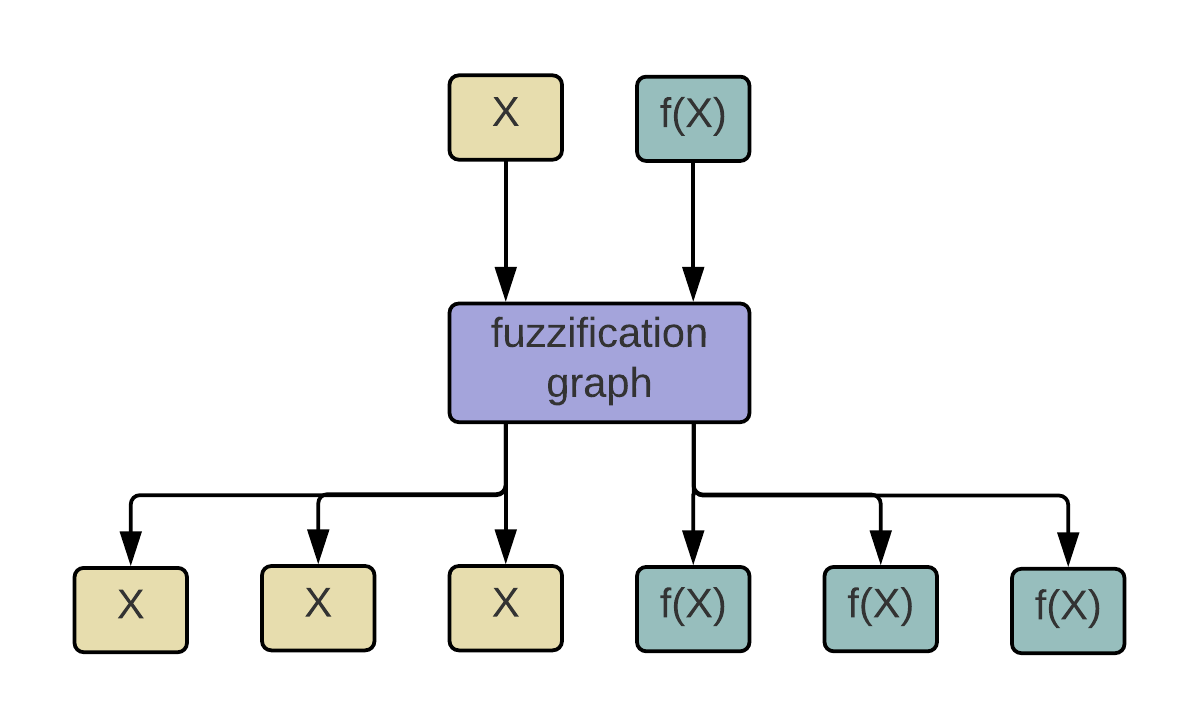
\includegraphics{fuzzification-graph}
	\caption[Ejemplo de operación de fuzzificación como grafo computacional]{Siendo el número de conjuntos difusos de las variables lingüísticas $X_1$ e $X_2$ $3$, el grafo de fuzzificación transformará los dos valores de entrada $x \in X_1$ e $y \in X_2$ en seis valores, los corerspondientes a los valores de pertenencia de $x$ e $y$ a cada uno de los conjuntos difusos de $X_1$ y $X_2$ respectivamente}
	\label{fig:fuzzification-graph}
\end{figure}

\newthought{La inferencia}, tomará esos valores difusos y generará los valores difusos de salida. Para ello, hará uso de un bloque de reglas en las que basará su inferencia.

Este bloque de reglas es el que se tratará de ajustar. La representación será la de una matriz $(v_i + 1)$-dimensional, siendo $v_i = \sum_{i=1}^l \left\vert{l_i}\right\vert$ (el número total de entradas difusas que llegan al bloque). La dimensión adicional se corresponde a la variable lingüística de salida.

Se puede pensar de esta manera. Para cada posible conjunto difuso de salida (es decir, para cada valor dentro del eje correspondiente a la salida), tenemos una matriz $v_i$-dimensional que se corresponde al producto cartesiano de las cariables de entradas. Esto es, cada una de las posibles combinaciones de reglas, a la que podemos asociar un valor. En la Figura~\ref{fig:inference-graph} se muestra un ejemplo con las variables obtenidas en el ejemplo de la Figura~\ref{fig:fuzzification-graph} tras aplicarles la $t$-norma.

\begin{figure}
	\centering
	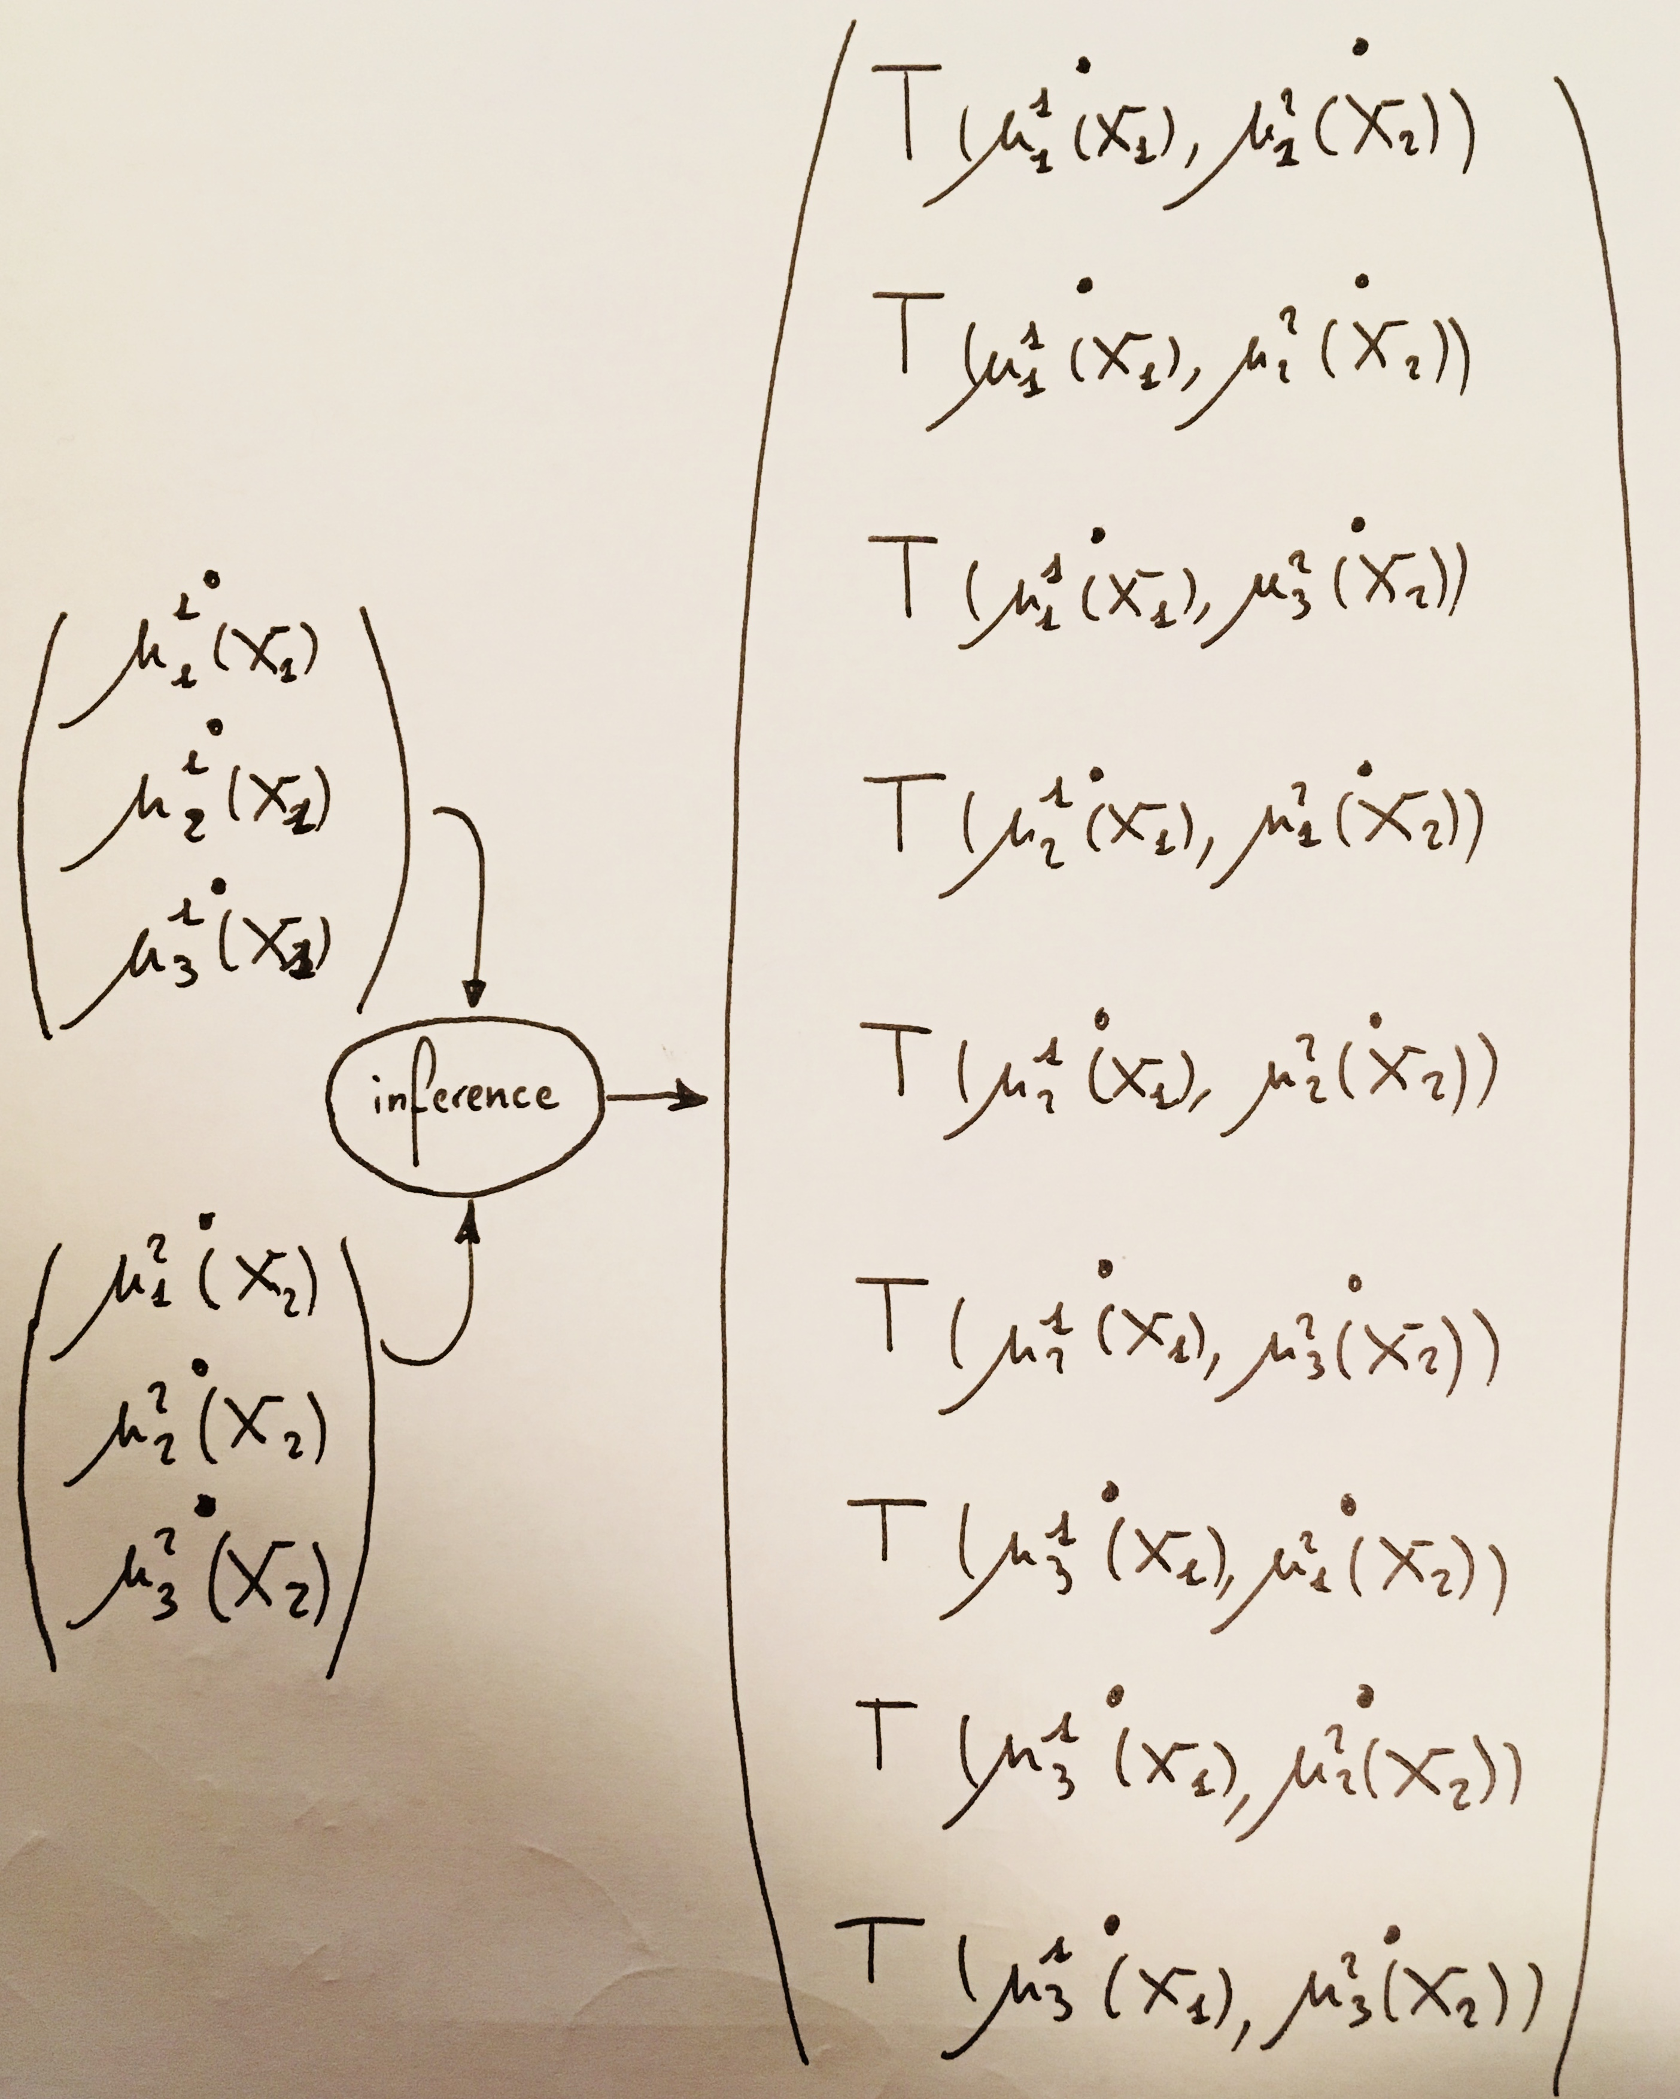
\includegraphics{inference-graph}
	\caption[Producto cartesiano de variables difusas de entrada]{El producto cartesiano de las variables difusas de entrada genera todas las posibles combinaciones entre los conjuntos difusos de las variables lingüísticas. Aplicándosele la $t$-norma a cada una de estas combinaciones tenemos todas las posibles reglas que se pueden definir en este \ac{fcs}.}
	\label{fig:inference-graph}
\end{figure}

Al estar definida la $t$-conorma y la acumulación con el mismo operador (i.e. el máximo), una regla de tipo OR es equivalente a dos reglas de tipo AND, ya que la acumulación de sus resultados es equivalente. Por tanto, al aplicar la $t$-norma a estas combinaciones tenemos todas las posibles combinaciones de reglas. Pero hasta aquí no tenemos ningún ajuste.

Si aplicamos el producto de hadamard contra una matriz de pesos con la misma dimensión y acotamos sus valores a $[0, 1] \in \mathbb{N}$, tenemos una manera de ajustar qué reglas son las más relevantes y cuáles no. Esta representación tiene un problema: las regiones definen meseta en la función de error, y por tanto en el momento que el gradiente cae en alguna de estas mesetas, la evolución de la variable se estanca. Sin embargo, si en lugar de un valor natural, el peso toma un valor real y le aplicamos una sigmoidal, el valor se mantendrá entre $(0, 1) \in \mathbb{R}$ con la ventaja de que el gradiente no se estanca, y en un proceso posterior se pueden descartar las reglas cuyos valores están próximos a $0$.

A la salida de la inferencia, tras aplicar la acumulación, disponemos de tantos valores difusos como conjuntos difusos tiene la salida.

\newthought{El último paso, la defuzzificación}, es una aplicación similar a las funciones de pertenencia, pero aquí no cabe lugar a ningún ajuste de variables.

De los valores difusos se obtiene un valor que será el correspondiente a la salida de nuestro \ac{fcs}.

\newthought{}
 
\TODO{Describir cómo se realiza la representación para el descenso del gradiente. Poner cosas con el ``algorithms'' si hace falta o queda guay, pero creo que mola más poner productos de matrices, tensores, etcétera. Poner también los dibujitos de los grafos, que molan mil.}

\TODO{Describir las decisiones durante el proceso de entrenamiento. Comparar diferentes aproximaciones de conjuntos difusos, poner las gráficas comparándolos y poner las reglas y las particiones difusas.}

\TODO{Describir epochs, tiempos de entrenamiento y de inferencia.}

\TODO{Separar los entrenamientos para todos los conductores y para los conductores en concreto. En estos últimos, si la red es muy grande, entrenar los modelos tanto desde 0 como desde una red preentrenada.}

\paragraph{Modelo \ac{mlp}}

\TODO{Describir el proceso de entrenamiento del controlador. Poner las grafiquitas de las diferentes arquitecturas usadas y selección de la mejor}

\TODO{Describir epochs, tiempos de entrenamiento y de inferencia.}

\TODO{Separar los entrenamientos para todos los conductores y para los conductores en concreto. En estos últimos, si la red es muy grande, entrenar los modelos tanto desde 0 como desde una red preentrenada.}

\paragraph{Comparación entre modelos}

\TODO{Sacar las gráficas para comparar sus RMS, decir cuál es el mejor e indicar que se usará ese.}

\subsection{Comportamiento en cambio de carril}

\TODO{Por hacer. Intuyo que habrá que separarlo en toma de decisión y cambio de carril.}

\TODO{Describir epochs, tiempos de entrenamiento y de inferencia.}

\TODO{Separar los entrenamientos para todos los conductores y para los conductores en concreto. En estos últimos, entrenar los modelos tanto desde 0 como desde una red preentrenada.}

\section{Validación del modelo}

\TODO{Para validar el modelo habrá que realizar una batería contra los conjuntos de test. Creo que la tasa de error en el problema de ajuste de la aceleración bale con un RMS, pero en el caso del cambio de carril habrá que indicar una tasa de acierto. Ésta debería tener en cuenta si cambiamos de carril dentro del tiempo estipulado para ello, en lugar de acertar directamente, pero si no pues ya lo apañaremos.}

\section{Implementación en entorno de simulación}

\TODO{Hablar de la implementación del lidar, de cómo se realiza la transformación someramente, un par de gráficas de la nube de puntos del entorno y del mapa de profundidad. Los vídeos para la presentación.}

-----------------------------------------------------------------

